\documentclass{article}

\usepackage{graphicx}
\usepackage{tikz}
\usepackage{tikzsymbols}
\usetikzlibrary{calc,patterns,shapes.geometric}
\pagestyle{empty}
\usepackage[margin=0pt]{geometry}
\geometry{papersize={14in,12in}}

\def\centerarc[#1](#2)(#3:#4:#5){\draw[#1] ($(#2)+({#5*cos(#3)},{#5*sin(#3)})$) arc (#3:#4:#5);}

\begin{document}
	\begin{figure}
		\centering
		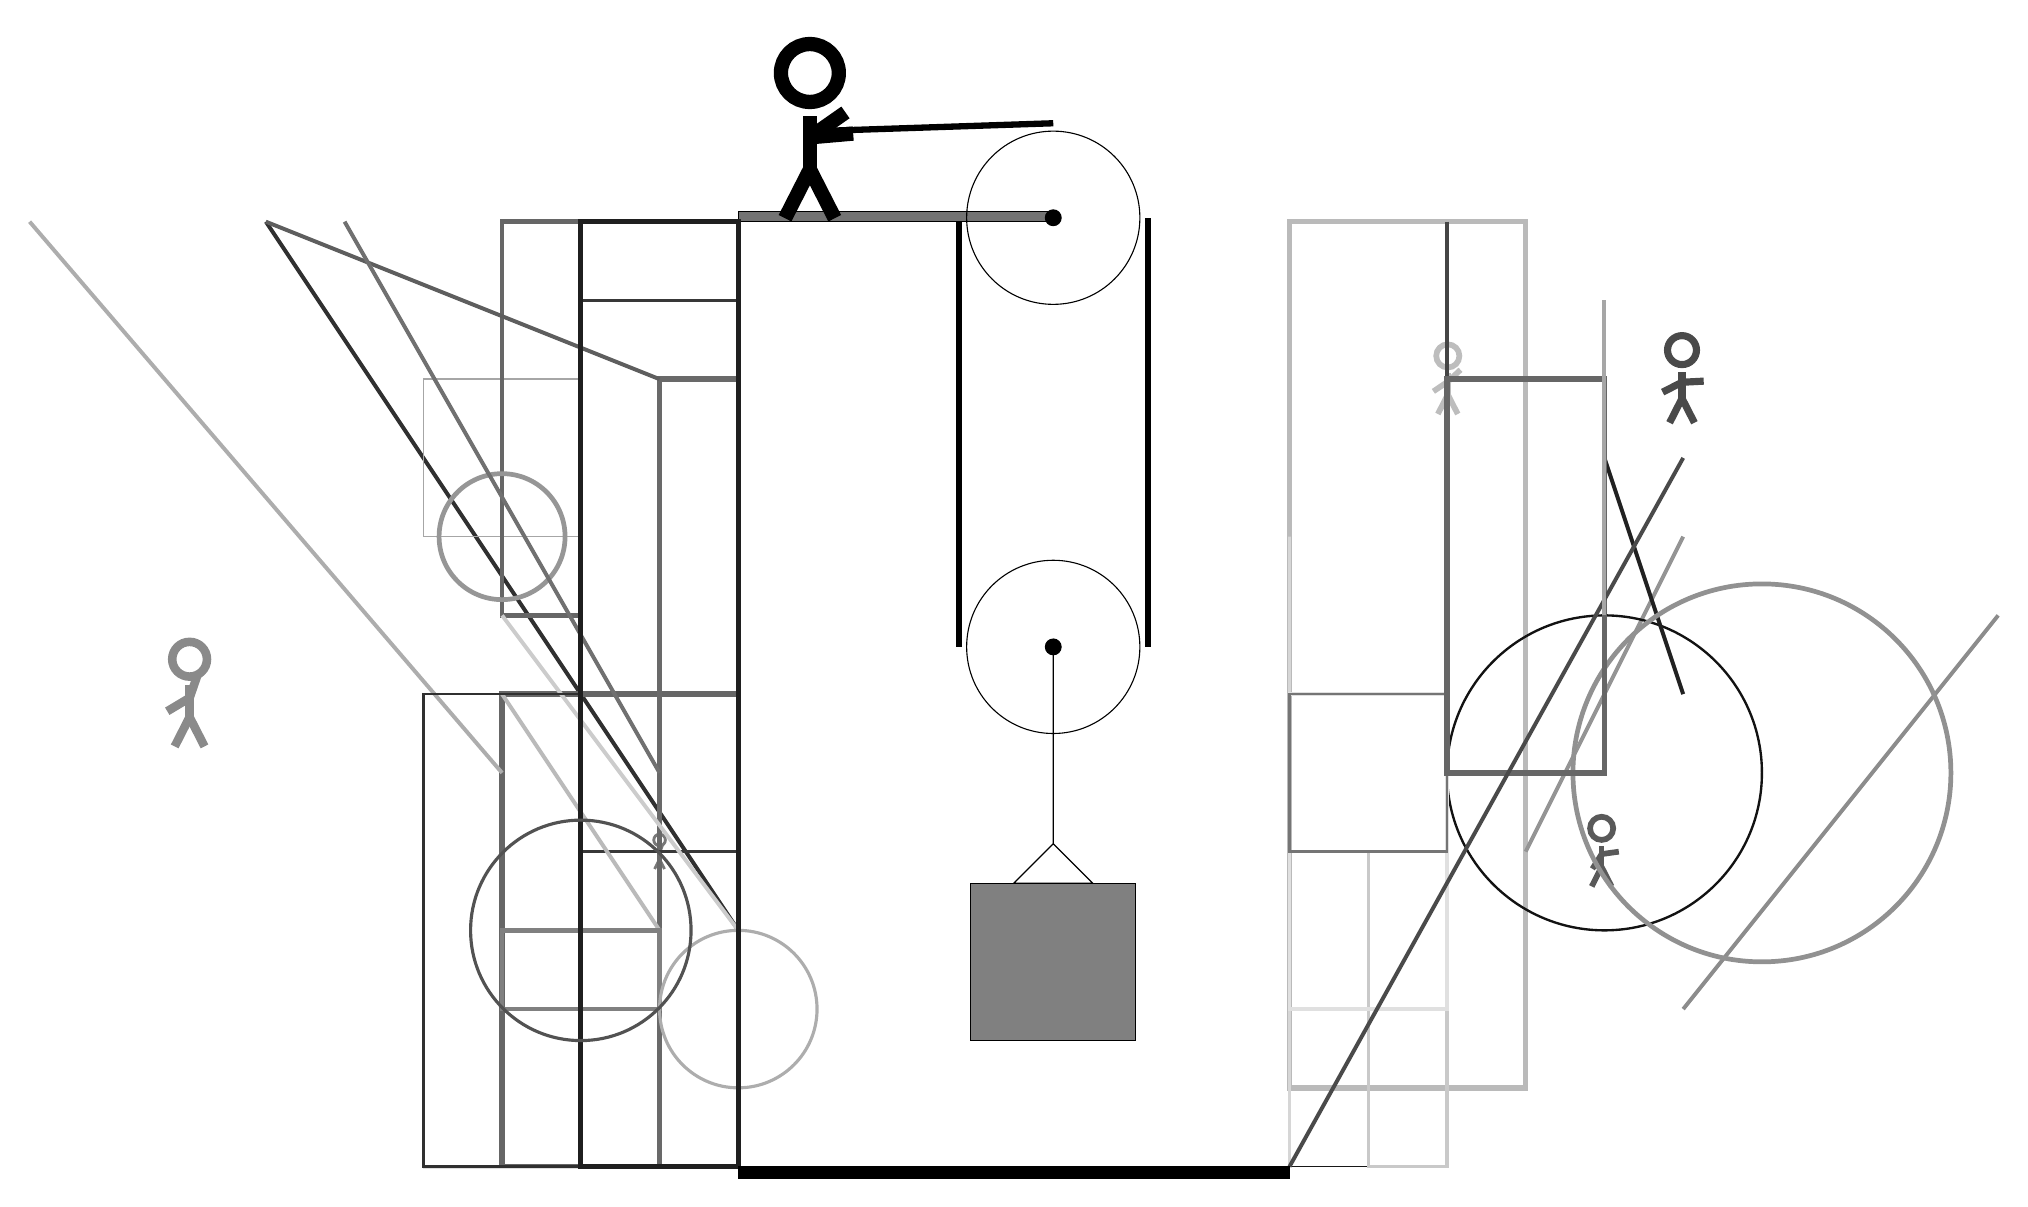
\begin{tikzpicture}
			%%%%% START %%%%%
			
			\draw[fill=black!55] (-2, 9) rectangle (2, 9.125);
			
			\draw (2, 3.6) circle (1.1);
			\draw[fill=black] (2, 3.6) circle (0.1);
			
			\draw[line width=0.7mm, color=black!27] (5, 9) rectangle (8, -2);
			
			\node[line width=0.6mm, color=black!46] at (-9, 3) {\Strichmaxerl[6][31][71]};
			\draw[line width=0.5mm, color=black!81](-2, 0) -- (-8, 9);
			\draw[line width=0.7mm, color=black!60] (-2, -3) rectangle (-5, 3);
			\node[line width=0.2mm, color=black!26] at (7, 7) {\Strichmaxerl[4][34][43]};
			\draw[line width=0.5mm, color=black!42](8, 1) -- (10, 5);
			\node[line width=0.3mm, color=black!53] at (-3, 1) {\Strichmaxerl[2][83][69]};
			
			\draw[line width=0.2mm, color=black!35] (-4, 7) rectangle (-6, 5);
			\draw[line width=0.6mm, color=black!60] (-4, 9) rectangle (-5, 4);
			\draw[line width=0.7mm, color=black!59] (-2, -3) rectangle (-3, 7);
			\draw[line width=0.5mm, color=black!63](-3, 7) -- (-8, 9);
			\draw[line width=0.2mm, color=black!91] (6, -3) rectangle (5, 1);
			\draw[line width=0.5mm, color=black!45](10, -1) -- (14, 4);
			\draw[line width=0.4mm, color=black!78] (-4, 1) rectangle (-2, 8);
			\draw[line width=0.4mm, color=black!21] (6, 1) rectangle (7, -3);
			\draw[line width=0.4mm, color=black!16] (5, 5) rectangle (5, -3);
			
			\draw[line width=0.5mm, color=black!20](-5, 4) -- (-2, 0);
			\draw [line width=0.3mm, color=black!93](9, 2) circle (2.0);
			\draw[line width=0.5mm, color=black!12] (7, -1) rectangle (5, 3);
			\node[line width=0.6mm, color=black!71] at (10, 7) {\Strichmaxerl[5][27][3]};
			\node[line width=0.3mm, color=black!65] at (9, 1) {\Strichmaxerl[4][58][8]};
			
			\draw[line width=0.5mm, color=black!27](-5, 3) -- (-3, 0);
			\draw[line width=0.5mm, color=black!32](-5, 2) -- (-11, 9);
			\draw[line width=0.5mm, color=black!13](-6, -3) -- (-2, -3);
			\draw[line width=0.6mm, color=black!50] (-3, 0) rectangle (-5, -1);
			
			\draw[line width=0.5mm, color=black!87](9, 6) -- (10, 3);
			
			\draw [line width=0.6mm, color=black!41](-5, 5) circle (0.8);
			\draw[line width=0.3mm, color=black!54] (5, 1) rectangle (7, 3);
			
			\draw[line width=0.5mm, color=black!56](-3, 2) -- (-7, 9);
			\draw [line width=0.4mm, color=black!32](-2, -1) circle (1.0);
			\draw[line width=0.3mm, color=black!81] (-4, 3) rectangle (-6, -3);
			
			\draw[line width=0.6mm, color=black!88] (-4, -3) rectangle (-2, 9);
			\draw [line width=0.6mm, color=black!43](11, 2) circle (2.4);
			
			\draw[line width=0.5mm, color=black!73](7, 9) -- (7, 5);
			\draw[line width=0.7mm, color=black!60] (7, 2) rectangle (9, 7);
			\draw [line width=0.4mm, color=black!68](-4, 0) circle (1.4);
			\draw[line width=0.5mm, color=black!71](10, 6) -- (5, -3);
			
			\draw[line width=0.5mm, color=black!35](9, 4) -- (9, 8);
			
			\draw (2, 9.05) circle (1.1);
			\draw[fill=black] (2, 9.05) circle (0.1);
			
			\draw (2, 3.6) -- (2, 1.1) -- (1.5, 0.6) -- (2.5, 0.6) -- (2, 1.1);
			\draw[fill=black!50] (0.95, 0.6) rectangle (3.05, -1.4);
			
			\draw[line width=0.8mm] (0.8, 9) -- (0.8, 3.6);
			\centerarc[line width=0.8mm](2, 3.6)(180:360:1.2000000000000002);
			\draw[line width=0.8mm](3.2, 3.6) -- (3.2, 9.05);
			\centerarc[line width=0.8mm](2, 9.05)(0:90:1.2000000000000002);
			\draw[line width=0.8mm](2, 10.25) -- (-1, 10.15);
			
			\node at (-1, 10.15) {\Strichmaxerl[10][-175][35]};
			
			\draw[fill=black] (-2, -3) rectangle (5, -3.15);
			
			%%%%% END %%%%%
		\end{tikzpicture}
	\end{figure}	
\end{document}